\chapter{Isosurface extraction with Marching Cubes}
\label{chap:marchingcubes}

This chapter will present a method of isosurface extraction that is later used
in the programming project. First, basic definitions will be established and
rationale for generating graphics with volumetric data will be discussed.
Next, brief history and high level overview of Marching Cubes will be presented.
Technical details will follow with description of implementation on highly
parallel GPGPU systems with OpenCL.

\section{Definitions}

\begin{defn}
\label{def:density function}
\emph{Density function} is a scalar function of the form
$\mathbb{R}^3\rightarrow\mathbb{R}$ or $\mathbb{R}^2\rightarrow\mathbb{R}$
that defines value of some magnitude in a continuous space. An example of such
function in 3D space is temperature defined in each point in the space. Height
on a flat map on the other hand is a density function in 2D space.

Note that such defined density function doesn't have any connection to
\emph{probability density function}. It's in fact a special kind of
\emph{scalar field}. This definition however is commonly used in context of
rendering isosurfaces \parencite{gpugems3ch01}.
\end{defn}

\begin{defn} \emph{Isosurface} is a
surface in three-dimensional space that consists of points that have the same
value of \emph{density function}.
Points
in domain which density function value is below this value are considered to
lie below the surface and points which density function value is above this
value are considered to lie above the surface. Points which density function
value is equal to the isovalue are considered to lie exactly on the isosurface.
\end{defn}

\begin{defn} \emph{Isovalue} is a value of density function that forms the
  \emph{isosurface}.
\end{defn}

\section{Rationale for isosurface rendering}

There are many applications which yield data as a density function. Some of them
are listed below:
\begin{description}
	\item[CT\footnotemark scan.]\footnotetext{Computer Tomography}
		Result of such scan is a set of 2D slices with each slice
		consisting of array of scalar values \parencite{Lorensen:1987:MCH:37402.37422}.
	\item[Weather data]
		Weather data, especially coming from weather models consists of
		scalar values of various parameters (temperature, humidity, etc.)
		on earth's surface
	\item[Arbitrary mathematical function]
		It's often desirable to visualise mathematical function with
		multiple parameters on 2D and 3D plots. For example for
		educational purposes.
	\item[Procedural models]
		Surfaces expressed by density function may be a source of
		visually interesting models that could be hard to model by hand.
\end{description}

Interactive presentation of such data may be very helpful while working with
these applications. Ability to rotate, zoom and scale such surfaces is
beneficial to understanding the data since human sight apparatus is naturally
well equipped to process 3D objects and images.

\section{Marching Cubes algorithm overview}
\subsection{History \parencite{mchist}}
Marching Cubes algorithm was invented in 1984 by William E. Lorensen and Harvey
E. Cline. While being employed by General Electric they attended a seminar by
GE's Medical Systems Business Group employee Carl Crawford. Mr Crawford
described capabilities of the upcoming rendering engine called \emph{Graphicon},
that rendered using polygons. He also challenged seminar attendees to find
interesting usages for the device. Within a day Lorenson and Cline devised an
algorithm that read volumetric medical data (essentially a density function) and
produced triangle mesh representing isosurface.

General Electric submitted a patent application for the algorithm on
June~5, 1985, which was granted on December~1, 1987 \parencite{mcpatent}.

Partly due to existence of this patent, another algorithm called
\emph{Marching Tetrahedra} was invented to give graphics community another
method of isosurface extraction, that is not encumbered by patents.
\emph{Marching Tetrahedra} also solves some ambiguities that are present in
\emph{Marching Cubes}.

Patent on \emph{Marching Cubes} algorithm expired in 2005.

\subsection{Algorithm description \parencite{Lorensen:1987:MCH:37402.37422}}
\label{sec:mcdesc}

Marching cubes algorithm divides space on which it operates into a discrete
lattice of cubes (interchangeably called \emph{voxels}). For each cube, density
function value is retrieved for each vertex of the cube. Density function may be
calculated from the position of the vertex on the fly if it's defined as a
mathematical function, or it may be extracted from some external volumetric data
source (e.g. result of CT scan).

Next, for each vertex of the cube it's determined whether value at its position
is larger or smaller than requested isovalue. If the value on the vertex is
smaller vertex is below the surface. Otherwise it's above it.

Being above or below the surface will be called the \emph{sign} of the vertex.
If vertices on the ends of given cube's edge are of different signs, than it's
certain that the surface crosses the edge.

For each cube, there are $2^8=256$ possible combinations of sings of the
vertices. Combination of these signs is called the
\emph{index} of this cube (see \autoref{fig:mcnumbering}).

When the index of the cube is known, pre-generated LUTs\footnote{Look-Up Tables}
are consulted to determine how many polygons and in what configuration should be
emitted for this cube.

Original version of Marching Cubes algorithm divides all 256 possible
combinations of vertices into 15 cases. These cases are presented in
\autoref{fig:mccases}. Remaining combinations are derived from these cases
through applying symmetries, rotations, and switching all signs of cube verices.

Process is repeated for all cubes in the lattice and emitted polygons (possibly
with normal vectors for lighting) are the output of the algorithm.

\begin{figure}[htb]
  \centerline{
    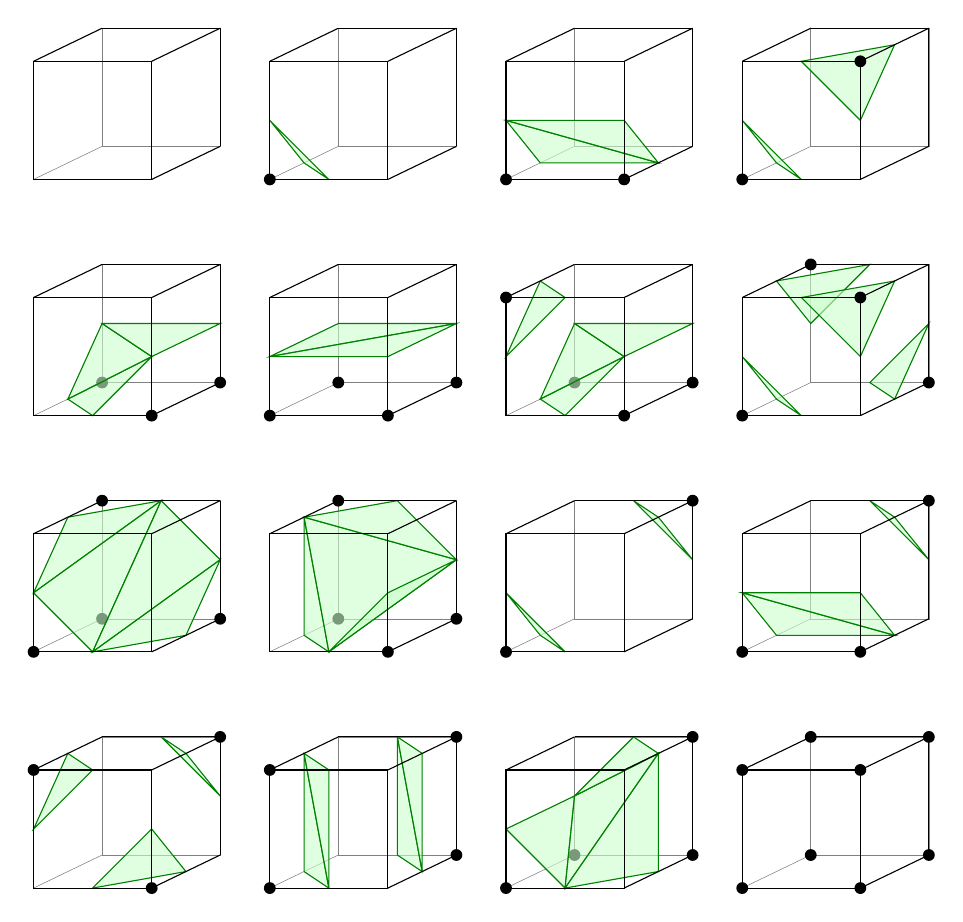
\begin{tikzpicture}[z={(-0.58cm,-0.28cm)}, scale=1.5]
      \tikzstyle{vertexfill} = [fill=green!20, fill opacity=0.6, draw=green!50!black]

  \def\cubeback{
    \draw[gray,very thin] +(0,0,-1) rectangle +(1,1,-1);
    \draw[gray,very thin] +(0,0,0) -- +(0,0,-1);
  }
  \def\cubefront{
    \draw +(1,0,-1) -- +(1,1,-1);
    \draw +(0,1,-1) -- +(1,1,-1);
    \draw +(0,0,0) rectangle +(1,1,0);
    \draw +(0,1,0) -- +(0,1,-1);
    \draw +(1,0,0) -- +(1,0,-1);
    \draw +(1,1,0) -- +(1,1,-1);
  }

  \begin{scope}[shift={(0,0)}]
    \cubeback
    \cubefront
  \end{scope}

  \begin{scope}[shift={(2,0)}]
    \cubeback
    \filldraw[vertexfill]
      (0,0.5,0) -- (0,0,-0.5) -- (0.5,0,0) -- cycle;
    \fill (0,0) circle (0.05);
    \cubefront
  \end{scope}

  \begin{scope}[shift={(4,0)}]
    \cubeback
    \filldraw[vertexfill]
      (0,0,-0.5) -- (0,0.5,0) -- (1,0,-0.5) -- cycle;
    \filldraw[vertexfill]
      (0,0.5,0) -- (1,0.5,0) -- (1,0,-0.5) -- cycle;
    \fill (0,0) circle (0.05);
    \fill (1,0) circle (0.05);
    \cubefront
  \end{scope}

  \begin{scope}[shift={(6,0)}]
    \cubeback
    \filldraw[vertexfill]
      (0,0.5,0) -- (0,0,-0.5) -- (0.5,0,0) -- cycle;
    \filldraw[vertexfill]
      (1,0.5,0) -- (1,1,-0.5) -- (0.5,1,0) -- cycle;
    \fill (0,0) circle (0.05);
    \fill (1,1) circle (0.05);
    \cubefront
  \end{scope}
  \begin{scope}[shift={(0,-2)}]
    \cubeback
    \fill (0,0,-1) circle (0.05);
    \filldraw[vertexfill]
      (0,0,-0.5) -- (0.5,0,0) -- (1,0.5,0) -- cycle;
    \filldraw[vertexfill]
      (0,0,-0.5) -- (0,0.5,-1) -- (1,0.5,0) -- cycle;
    \filldraw[vertexfill]
      (1,0.5,0) -- (1,0.5,-1) -- (0,0.5,-1) -- cycle;
    
    \fill (1,0) circle (0.05);
    \fill (1,0,-1) circle (0.05);
    \cubefront
  \end{scope}
  \begin{scope}[shift={(2,-2)}]
    \cubeback
    \filldraw[vertexfill]
      (0,0.5,0) -- (1,0.5,-1) -- (0,0.5,-1) -- cycle;
    \filldraw[vertexfill]
      (0,0.5,0) -- (1,0.5,0) -- (1,0.5,-1) -- cycle;

    \fill (0,0) circle (0.05);
    \fill (1,0) circle (0.05);
    \fill (1,0,-1) circle (0.05);
    \fill (0,0,-1) circle (0.05);
    \cubefront
  \end{scope}
  \begin{scope}[shift={(4,-2)}]
    \cubeback
    \fill (0,0,-1) circle (0.05);
    \filldraw[vertexfill]
      (0,0.5,0) -- (0.5,1,0) -- (0,1,-0.5) -- cycle;
    \filldraw[vertexfill]
      (0,0,-0.5) -- (0.5,0,0) -- (1,0.5,0) -- cycle;
    \filldraw[vertexfill]
      (0,0,-0.5) -- (0,0.5,-1) -- (1,0.5,0) -- cycle;
    \filldraw[vertexfill]
      (1,0.5,0) -- (1,0.5,-1) -- (0,0.5,-1) -- cycle;

    \fill (0,1,0) circle (0.05);
    \fill (1,0) circle (0.05);
    \fill (1,0,-1) circle (0.05);
    \cubefront
  \end{scope}
  \begin{scope}[shift={(6,-2)}]
    \cubeback
    \fill (0,1,-1) circle (0.05);
    \fill (1,0,-1) circle (0.05);
    \filldraw[vertexfill]
      (0,1,-0.5) -- (0,0.5,-1) -- (0.5,1,-1) -- cycle;
    \filldraw[vertexfill]
      (0,0.5,0) -- (0,0,-0.5) -- (0.5,0,0) -- cycle;
    \filldraw[vertexfill]
      (1,0.5,0) -- (1,1,-0.5) -- (0.5,1,0) -- cycle;
    \filldraw[vertexfill]
      (1,0,-0.5) -- (1,0.5,-1) -- (0.5,0,-1) -- cycle;

    \fill (1,1) circle (0.05);
    \fill (0,0) circle (0.05);
    \cubefront
  \end{scope}
  \begin{scope}[shift={(0,-4)}]
    \cubeback
    \fill (0,1,-1) circle (0.05);
    \fill (0,0,-1) circle (0.05);
    \fill (1,0,-1) circle (0.05);
    \filldraw[vertexfill]
      (0,0.5,0) -- (0.5,1,-1) -- (0,1,-0.5) -- cycle;
    \filldraw[vertexfill]
      (0,0.5,0) -- (0.5,0,0) -- (0.5,1,-1) -- cycle;
    \filldraw[vertexfill]
      (0.5,0,0) -- (1,0.5,-1) -- (0.5,1,-1) -- cycle;
    \filldraw[vertexfill]
      (0.5,0,0) -- (1,0,-0.5) -- (1,0.5,-1) -- cycle;
    \fill (0,0) circle (0.05);
    \cubefront
  \end{scope}
  \begin{scope}[shift={(2,-4)}]
    \cubeback
    \fill (0,0,-1) circle (0.05);
    \fill (1,0,-1) circle (0.05);
    \fill (0,1,-1) circle (0.05);

    \filldraw[vertexfill]
      (0,0,-0.5) -- (0.5,0,0) -- (0,1,-0.5) -- cycle;
    \filldraw[vertexfill]
      (0.5,0,0) -- (1,0.5,-1) -- (0,1,-0.5) -- cycle;
    \filldraw[vertexfill]
      (0.5,0,0) -- (1,0.5,0) -- (1,0.5,-1) -- cycle;
    \filldraw[vertexfill]
      (0,1,-0.5) -- (1,0.5,-1) -- (0.5,1,-1) -- cycle;

    \fill (1,0) circle (0.05);
    \cubefront
  \end{scope}
  \begin{scope}[shift={(4,-4)}]
    \cubeback
    \fill (1,1,-1) circle (0.05);
    \filldraw[vertexfill]
      (0,0.5,0) -- (0,0,-0.5) -- (0.5,0,0) -- cycle;
    \filldraw[vertexfill]
      (1,1,-0.5) -- (1,0.5,-1) -- (0.5,1,-1) -- cycle;
    \fill (0,0) circle (0.05);
    \cubefront
  \end{scope}
  \begin{scope}[shift={(6,-4)}]
    \cubeback
    \fill (1,1,-1) circle (0.05);
    \filldraw[vertexfill]
      (1,1,-0.5) -- (1,0.5,-1) -- (0.5,1,-1) -- cycle;
    \filldraw[vertexfill]
      (0,0,-0.5) -- (0,0.5,0) -- (1,0,-0.5) -- cycle;
    \filldraw[vertexfill]
      (0,0.5,0) -- (1,0.5,0) -- (1,0,-0.5) -- cycle;
    \fill (0,0) circle (0.05);
    \fill (1,0) circle (0.05);
    \cubefront
  \end{scope}
  \begin{scope}[shift={(0,-6)}]
    \cubeback
    \fill (1,1,-1) circle (0.05);
    \filldraw[vertexfill]
      (1,1,-0.5) -- (1,0.5,-1) -- (0.5,1,-1) -- cycle;
    \filldraw[vertexfill]
      (0,0.5,0) -- (0.5,1,0) -- (0,1,-0.5) -- cycle;
    \filldraw[vertexfill]
      (0.5,0,0) -- (1,0,-0.5) -- (1,0.5,0) -- cycle;

    \fill (1,0,0) circle (0.05);
    \fill (0,1,0) circle (0.05);
    \cubefront
  \end{scope}
  \begin{scope}[shift={(2,-6)}]
    \cubeback
    \fill (1,1,-1) circle (0.05);
    \fill (1,0,-1) circle (0.05);

    \filldraw[vertexfill]
      (0,0,-0.5) -- (0.5,0,0) -- (0,1,-0.5) -- cycle;
    \filldraw[vertexfill]
      (0,1,-0.5) -- (0.5,0,0) -- (0.5,1,0) --  cycle;
    \filldraw[vertexfill]
      (1,0,-0.5) -- (0.5,1,-1) -- (0.5,0,-1) -- cycle;
    \filldraw[vertexfill]
      (1,0,-0.5) -- (1,1,-0.5) -- (0.5,1,-1) -- cycle;

    \fill (0,0,0) circle (0.05);
    \fill (0,1,0) circle (0.05);
    \cubefront
  \end{scope}
  \begin{scope}[shift={(4,-6)}]
    \cubeback
    \fill (0,0,-1) circle (0.05);
    \fill (1,1,-1) circle (0.05);
    \fill (1,0,-1) circle (0.05);

    \filldraw[vertexfill]
      (0,0.5,0) -- (0.5,0,0) -- (0,0.5,-1) -- cycle;
    \filldraw[vertexfill]
      (0.5,0,0) -- (1,1,-0.5) -- (0,0.5,-1) -- cycle;
    \filldraw[vertexfill]
      (0.5,0,0) -- (1,0,-0.5) -- (1,1,-0.5) -- cycle;
    \filldraw[vertexfill]
      (1,1,-0.5) -- (0.5,1,-1) -- (0,0.5,-1) -- cycle;

    \fill (0,0,0) circle (0.05);
    \cubefront
  \end{scope}
  \begin{scope}[shift={(6,-6)}]
    \cubeback
    \fill (0,0,0) circle (0.05);
    \fill (0,0,-1) circle (0.05);
    \fill (0,1,0) circle (0.05);
    \fill (0,1,-1) circle (0.05);
    \fill (1,0,0) circle (0.05);
    \fill (1,0,-1) circle (0.05);
    \fill (1,1,0) circle (0.05);
    \fill (1,1,-1) circle (0.05);
    \cubefront
  \end{scope}

    \end{tikzpicture}
  }
  \caption{
    All cases in traditional Marching cubes algorithm. Vertices with density
    function above threshold value have black circles on them. Symmetries,
    rotations, and complementary cases (with exception of cases 0 and 255) were
    omitted for brevity.
  }
  \label{fig:mccases}
\end{figure}

\subsubsection{Cube indexing}

Operation on a single cube begins with evaluating density function on each
vertex of the cube.

Index of the cube is calculated through operation described below
\autoref{fig:mcnumbering}.

\begin{figure}[hb]
  \centerline{
   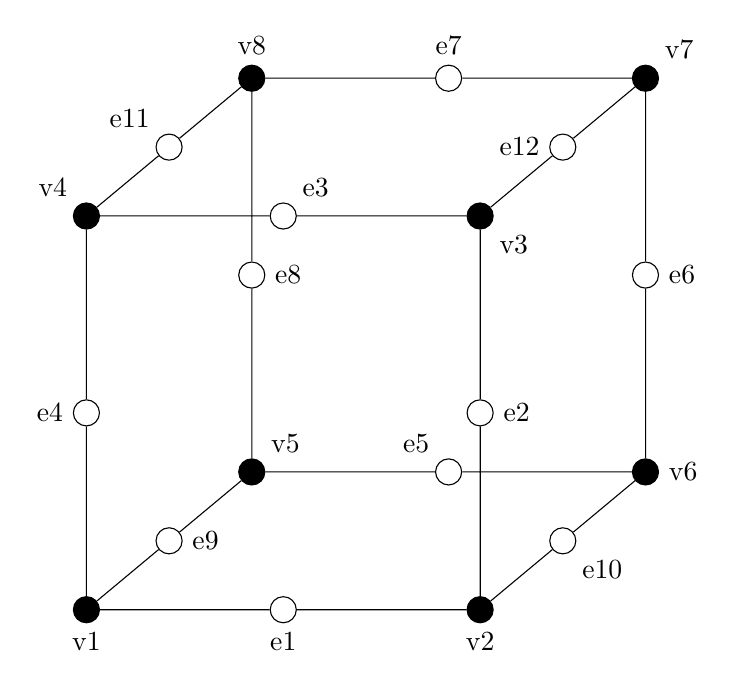
\begin{tikzpicture}[
  z={(-0.42cm,-0.35cm)}, scale=2.5,
  vert/.style={circle,draw=black,fill=black},
  edge/.style={circle,draw=black,fill=white}
]
 
  \node at (0,0,0) [vert,label=below:v1] (v1) {};
  \node at (1,0,0) [edge,label=below:e1] (e1) {};
  \node at (2,0,0) [vert,label=below:v2] (v2) {};
  \node at (2,1,0) [edge,label=right:e2] (e2) {};
  \node at (2,2,0) [vert,label=south east:v3] (v3) {};
  \node at (1,2,0) [edge,label=north east:e3] (e3) {};
  \node at (0,2,0) [vert,label=north west:v4] (v4) {};
  \node at (0,1,0) [edge,label=left:e4] (e4) {};
  \node at (0,0,-2) [vert,label=north east:v5] (v5) {};
  \node at (1,0,-2) [edge,label=north west:e5] (e5) {};
  \node at (2,0,-2) [vert,label=right:v6] (v6) {};
  \node at (2,1,-2) [edge,label=right:e6] (e6) {};
  \node at (2,2,-2) [vert,label=north east:v7] (v7) {};
  \node at (1,2,-2) [edge,label=above:e7] (e7) {};
  \node at (0,2,-2) [vert,label=above:v8] (v8) {};
  \node at (0,1,-2) [edge,label=right:e8] (e8) {};
  \node at (0,0,-1) [edge,label=right:e9] (e9) {};
  \node at (2,0,-1) [edge,label=south east:e10] (e10) {};
  \node at (2,2,-1) [edge,label=left:e12] (e12) {};
  \node at (0,2,-1) [edge,label=north west:e11] (e11) {};

  \draw
    (v1) -- (e1) -- (v2) -- (e2) -- (v3) -- (e3) -- (v4) -- (e4) -- (v1)
    (v5) -- (e5) -- (v6) -- (e6) -- (v7) -- (e7) -- (v8) -- (e8) -- (v5)
    (v1) -- (e9) -- (v5)
    (v2) -- (e10) -- (v6)
    (v4) -- (e11) -- (v8)
    (v3) -- (e12) -- (v7);
\end{tikzpicture}

  }
  \caption{
    Numbering of vertices and edges in Marching Cubes. Cube index is
    derived by concatenation of bits \texttt{index = v8|v7|v6|v5|v4|v3|v2|v1}
    where each \texttt{v}\emph{i} is logical result (0 or 1) of operation of comparing
    density function value at \emph{i}-th vertex with threshold value
    (\texttt{value(i) > threshold}).
  }
  \label{fig:mcnumbering}
\end{figure}

\subsubsection{Emitting polygons}
\label{sec:mcemitting}

When index of the cube is known, LUT is consulted that maps index to list of
edges on which vertex in given cube must be emitted.

\begin{lstlisting}[caption={Index to edge list LUT. Notice that for indices 0
and 255 no geometry is emitted}]
unsigned char mcTriangleTable[256][16] = {
        {255, 255, 255, 255, 255, 255, 255, 255, 255, 255, 255, 255, 255, 255, 255, 255},
        {0, 8, 3, 255, 255, 255, 255, 255, 255, 255, 255, 255, 255, 255, 255, 255},
        ...
        {0, 3, 8, 255, 255, 255, 255, 255, 255, 255, 255, 255, 255, 255, 255, 255},
        {255, 255, 255, 255, 255, 255, 255, 255, 255, 255, 255, 255, 255, 255, 255, 255}
};
\end{lstlisting}

For each edge on the list vertex is emitted between its two ends in place
proportional to the linear interpolation of density function at the vertices.

Each three vertices form a polygon. In the listing above, value 255 marks an end
of the list for given index.

Next, each polygon is saved in a list for later usage, or directly fed to
rendering device.

\section{Implementation on GPU with OpenCL}
\label{sec:mcgpu}
Following implementation is based on example code from NVIDIA CUDA SDK
example\footnote{\url{http://docs.nvidia.com/cuda/cuda-samples/index.html\#marching-cubes-isosurfaces}}.

As described in \autoref{sec:mcdesc} each cube is processed by the algorithm
independently. This possibly makes this algorithm a good candidate for massive
parallelization offered by general purpose GPU programming. There are however
some obstacles to overcome.

First, LUTs used by the algorithm are obviously too big to fit into registers.
Reading them from global memory would also be problematic, because they are
accessed in a random manner, depending on cube index. Tables could be copied
to local memory for faster access, but the cost of copying for each block could
be substantial.

Another problem is storage of the output. It is not known beforehand how many
polygons will be emitted by each cube. With sequential implementation it isn't a
problem because data generated by each cube may be just appended to single
result array. With many cubes being process at the same time, this approach
will not work.

\subsection{Stages in GPU implementation}
Kernel execution is divided into the following stages:
\begin{enumerate}
  \item voxel classification
  \item compacting
  \item triangle generation
\end{enumerate}

All operations are performed on cube lattice flattened to 1D array. Each stage
of the execution will be described below.

\subsubsection{Voxel classification}

In this stage, all voxels are classified as to whether they will produce any
geometry or not, and how many vertices is given voxel going to produce.

Results are written to two arrays: \texttt{voxelOccupied} which contains 1
if given voxel produces any geometry and 0 otherwise, and
\texttt{voxelVerts} that holds number of vertices produced by this voxel:
\todo{Find out about having single listing with some dialect}
\begin{lstlisting}[language=opencl, numbers=left]
__kernel
void classifyVoxel(
	__global uint *voxelVerts,
	__global uint *voxelOccupied,
	uint4 gridSize,
	float4 voxelSize,
	float isoValue,
	uint numVoxels,
	__read_only image2d_t numVertsTex)
{
	uint i = get_global_id(0);
	float4 cubeValues[8];
	/* Here, values on each vertex of the voxel are inserted into cubeValues array */

	int cubeIndex = getCubeIndex(cubeValues, isoValue);
	uint numVerts = read_imageui(numVertsTex, tableSampler, (int2)(cubeIndex, 0)).x;
	if (i < numVoxels) {
		voxelVerts[i] = numVerts;
		voxelOccupied[i] = (numVerts > 0);
	}
}
\end{lstlisting}
Note that additional lookup table (\texttt{numVertsTex}) that maps cube index to
number of vertices it produces is used. This LUT is accessed as a texture.

Index of the cube is calculated as described in \autoref{fig:mcnumbering}:

\begin{lstlisting}
int getCubeIndex(float4 *cubeValues, float isoValue)
{
	int cubeIndex;
	cubeIndex =  (cubeValues[0].w < isoValue);
	cubeIndex += (cubeValues[1].w < isoValue) << 1;
	cubeIndex += (cubeValues[2].w < isoValue) << 2;
	/*...*/
	cubeIndex += (cubeValues[7].w < isoValue) << 7;
	return cubeIndex;
}
\end{lstlisting}

\subsubsection{Compacting}

\begin{figure}[b]
	\begin{center}
		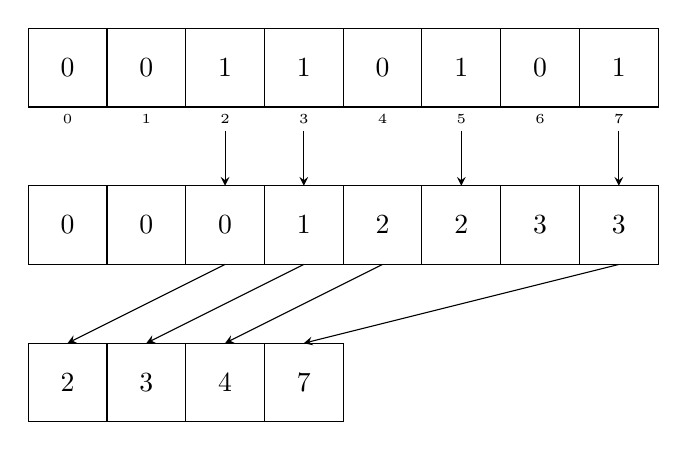
\begin{tikzpicture}[>=stealth]

\foreach \x/\val in {0/0,1/0,2/1,3/1,4/0,5/1,6/0,7/1}
{
  \draw (\x,0) rectangle ++(1,1);
  \draw node at (\x+0.5,0.5) {\val};
  \draw[font=\tiny] node at (\x+0.5,-0.15) {\x};
}

\foreach \x in {2,3,5,7}
{
  \draw[->] (\x+0.5,-0.3) -- ++(0,-0.7);
}

\foreach \x/\val in {0/0,1/0,2/0,3/1,4/2,5/2,6/3,7/3}
{
  \draw (\x,-2) rectangle ++(1,1);
  \draw node at (\x+0.5,-1.5) {\val};
}

\foreach \x/\val in {0/2,1/3,2/4,3/7}
{
  \draw (\x,-4) rectangle ++(1,1);
  \draw node at (\x+0.5,-3.5) {\val};
}

\foreach \x/\y in {0/2,1/3,2/4,3/7}
{
  \draw[->] (\y+0.5,-2) -- (\x+0.5, -3);
}
\end{tikzpicture}
	\end{center}
	\caption{Example of compaction procedure. Index of each non empty voxel
		is saved in \texttt{compactedVoxelArray}. Place to which index
		should be stored is read from \texttt{voxelOccupiedScan} array.
	}
	\label{fig:mccompact}
\end{figure}

To overcome problem highlighted in \autoref{sec:mcgpu} a special compacting
operation is performed on arrays from previous step. First, a prefix-sum array
is computed in parallel on the GPU\footnote{Implementation based on \cite{gpugemsscan},
as included in \href{https://developer.nvidia.com/cuda-downloads}{NVIDIA CUDA SDK}}
on \texttt{voxelOccupied} and \texttt{voxelVerts} arrays resulting in
\texttt{voxelOccupiedScan} and \texttt{voxelVertsScan} arrays.

\begin{defn}[Prefix-sum operation \parencite{BlellochTR90}]
Operation that takes binary associative operator $\oplus$ with identity $I$ and
an array of $n$ elements $[a_0,a_1,\ldots,a_{n-1}]$ and returns the array
$[I,a_0,(a_0\oplus a_1),\ldots,(a_0\oplus a_1 \oplus \ldots \oplus a_{n-2})]$

This operation is sometimes called \emph{scan} operation.
\end{defn}

By reading the last elements of \texttt{voxelOccupied} and
\texttt{voxelOccupiedScan} and adding them, the number of voxels that will
produce geometry can be obtained. These voxels are called \emph{active voxels}.

Thanks to voxel compaction, the most computation--intensive kernel, i.e.
\texttt{generateTriangles} kernel that generates final geometry can be computed
only for voxels that are not empty. Since in many cases, space on which Marching
Cubes is working is rather sparse, this approach can bring enormous performance
gains.

Let call the number of active voxels $n$. Compaction kernel creates an array
of length $n$ that will contain indexes of non empty voxels. For illustration of
this process refer to \autoref{fig:mccompact}.

Below is the code that performs the compaction.
\begin{lstlisting}[language=opencl]
__kernel
void compactVoxels(
	__global uint *compactedVoxelArray,
	__global uint *voxelOccupied,
	__global uint *voxelOccupiedScan,
	uint numVoxels
)
{
	uint i = get_global_id(0);
	if(voxelOccupied[i] && (i < numVoxels)) {
		compactedVoxelArray[voxelOccupiedScan[i]] = i;
	}
}
\end{lstlisting}

Scan operation on \texttt{voxelVerts} array gives \texttt{generateTriangles}
kernel an offset to the result array where data for given voxel should be written.
For an example refer to \autoref{fig:mcvertscan}.

\begin{figure}[htb]
	\begin{center}
		%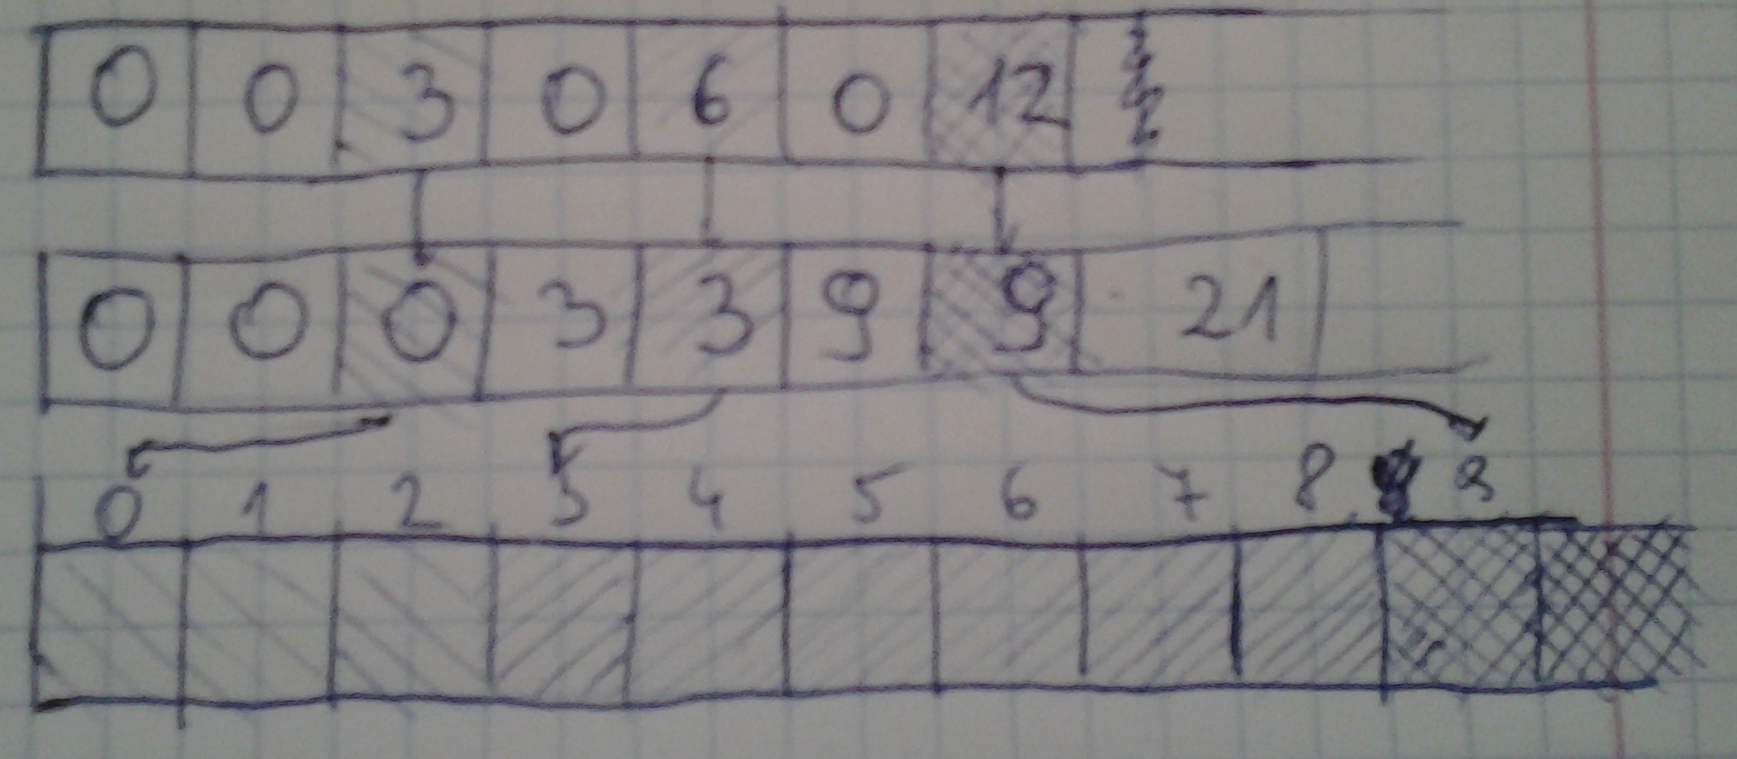
\includegraphics[width=\textwidth]{chapters/marchingcubes/vertscan.jpg}
		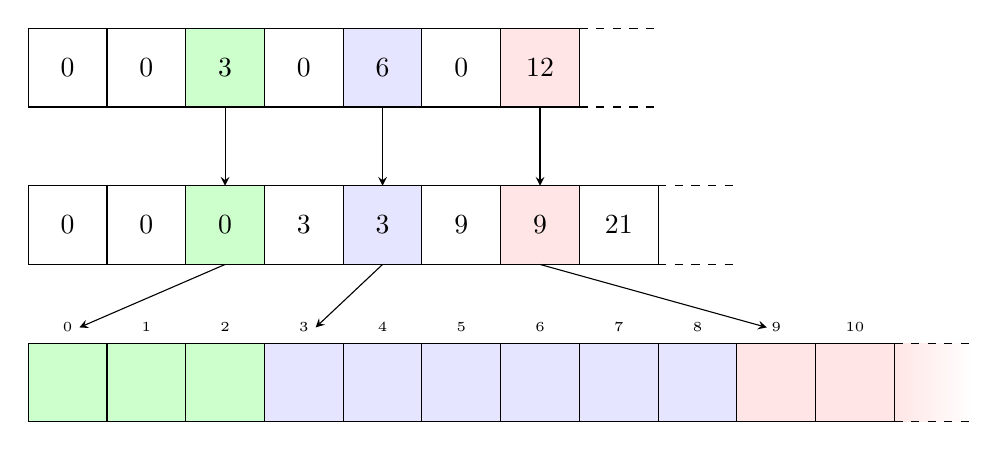
\begin{tikzpicture}[>=stealth]
\usetikzlibrary{fadings}

\draw[fill=green!20] (2,0) rectangle ++(1,1);
\draw[fill=blue!10] (4,0) rectangle ++(1,1);
\draw[fill=red!10] (6,0) rectangle ++(1,1);


\foreach \x/\val in {0/0,1/0,2/3,3/0,4/6,5/0,6/12}
{
  \draw (\x,0) rectangle ++(1,1);
  \draw node at (\x+0.5, 0.5) {\val};
}
\draw[dashed] (7,1) -- ++(1,0);
\draw[dashed] (7,0) -- ++(1,0);

\foreach \x in {2,4,6}
{
  \draw[->] (\x+0.5,0) -- ++(0,-1);
}

\draw[fill=green!20] (2,-2) rectangle ++(1,1);
\draw[fill=blue!10] (4,-2) rectangle ++(1,1);
\draw[fill=red!10] (6,-2) rectangle ++(1,1);

\foreach \x/\val in {0/0,1/0,2/0,3/3,4/3,5/9,6/9,7/21}
{
  \draw (\x,-2) rectangle ++(1,1);
  \draw node at (\x+0.5, -1.5) {\val};
}
\draw[dashed] (8,-1) -- ++(1,0);
\draw[dashed] (8,-2) -- ++(1,0);

\foreach \x in {0,...,2}
  \draw[fill=green!20] (\x,-4) rectangle ++(1,1);

\foreach \x in {3,...,8}
  \draw[fill=blue!10] (\x,-4) rectangle ++(1,1);

\foreach \x in {9,10}
  \draw[fill=red!10] (\x,-4) rectangle ++(1,1);

\fill [red!10,path fading=east] (11,-4) rectangle ++(1,1);

\draw[->] (2.5, -2) -- (0.65, -2.8);

\draw[->] (4.5, -2) -- (3.65, -2.8);
\draw[->] (6.5, -2) -- (9.38, -2.8);


\foreach \x in {0,...,10}
{
  \draw (\x,-4) rectangle ++(1,1);
  \draw[font=\tiny] node at (\x+0.5, -2.8) {\x};
}

\draw[dashed] (11,-3) -- ++(1,0);
\draw[dashed] (11,-4) -- ++(1,0);


\end{tikzpicture}
	\end{center}
	\caption{Scan operation on \texttt{voxelVerts} array gives indexes to
		final result array for every active voxel.
	}
	\label{fig:mcvertscan}
\end{figure}

\subsubsection{Generating triangles}

Triangle generation is handled by \texttt{generateTriangles} kernel. It figures
out the number of voxel it's working on from \texttt{compactedVoxelArray}. Next,
array in local memory is allocated for computing locations of vertices on each
of the 12 edges on the cube.

\begin{lstlisting}
__local float4 vertList[12*NTHREADS];
__local float4 normList[12*NTHREADS];
\end{lstlisting}

Positions are calculated even though certain edges may not have surface border
on them. However, using \texttt{if} statement in kernel in this context would
cause divergence in execution of parallel threads.

From now on, algorithm is the same as in sequential version. List of edges on
which vertices lie is read from LUT mentioned in \autoref{sec:mcemitting}. This
table is accessed as a 2D texture. Agressive caching strategy implemented in
GPUs for texture data access allows the kernel to retrieve the data without
much penalty. Positions of vertices and normals on edges read from LUT are read
from \texttt{vertList} and \texttt{normList} arrays, and are written into result
vertex position and normal arrays on indices read from \texttt{voxelVertsScan}
array.
